%!TEX root = ../main.tex

\section*{Results}

  \begin{figure}[h]
    \begin{center}
      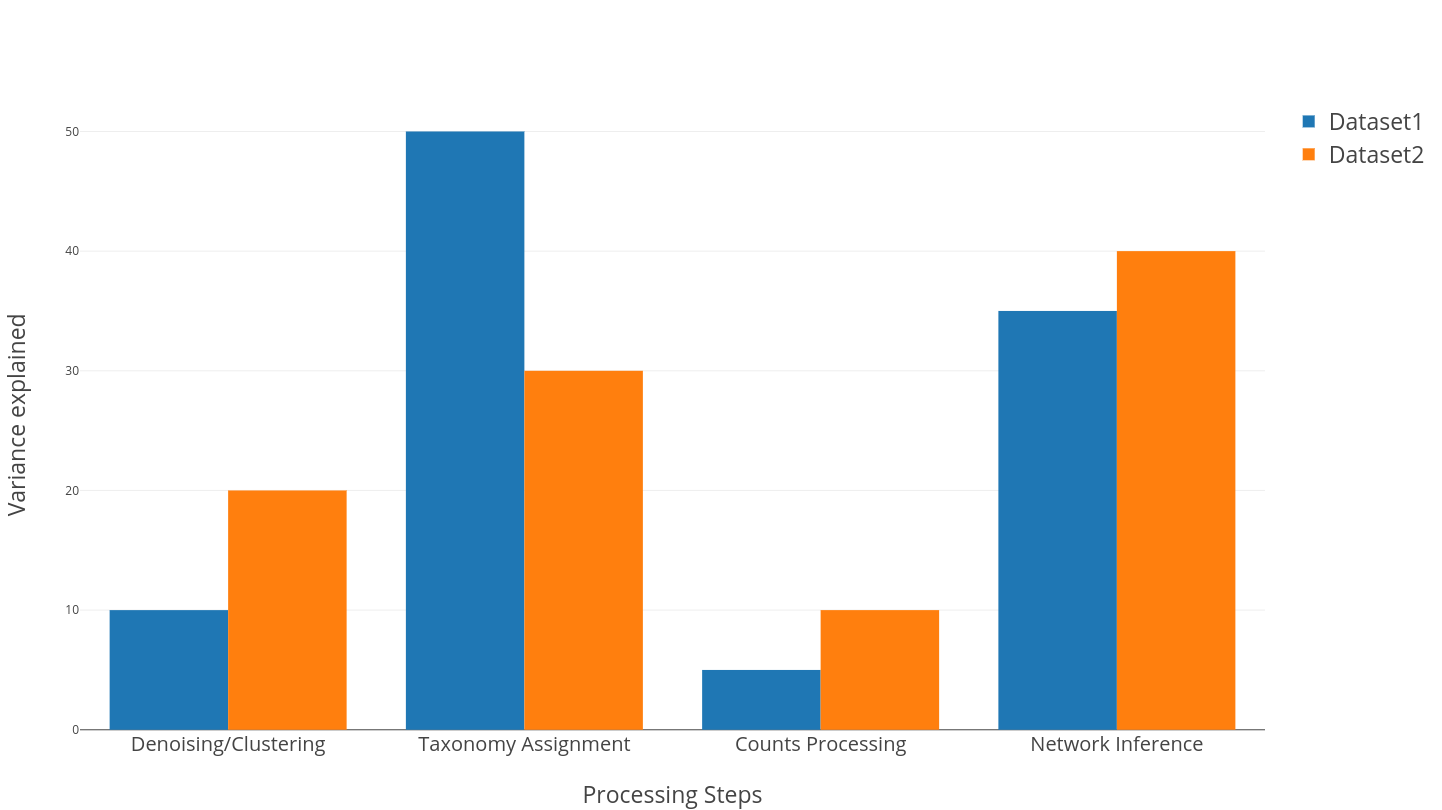
\includegraphics[width=17.8cm]{main_figure.png}
      \caption{\textbf{Percentage of variance in the final co-occurrence network due to each processing step.} }
      \label{fig:variance}
    \end{center}
  \end{figure}

  \begin{figure}[h]
    \begin{center}
      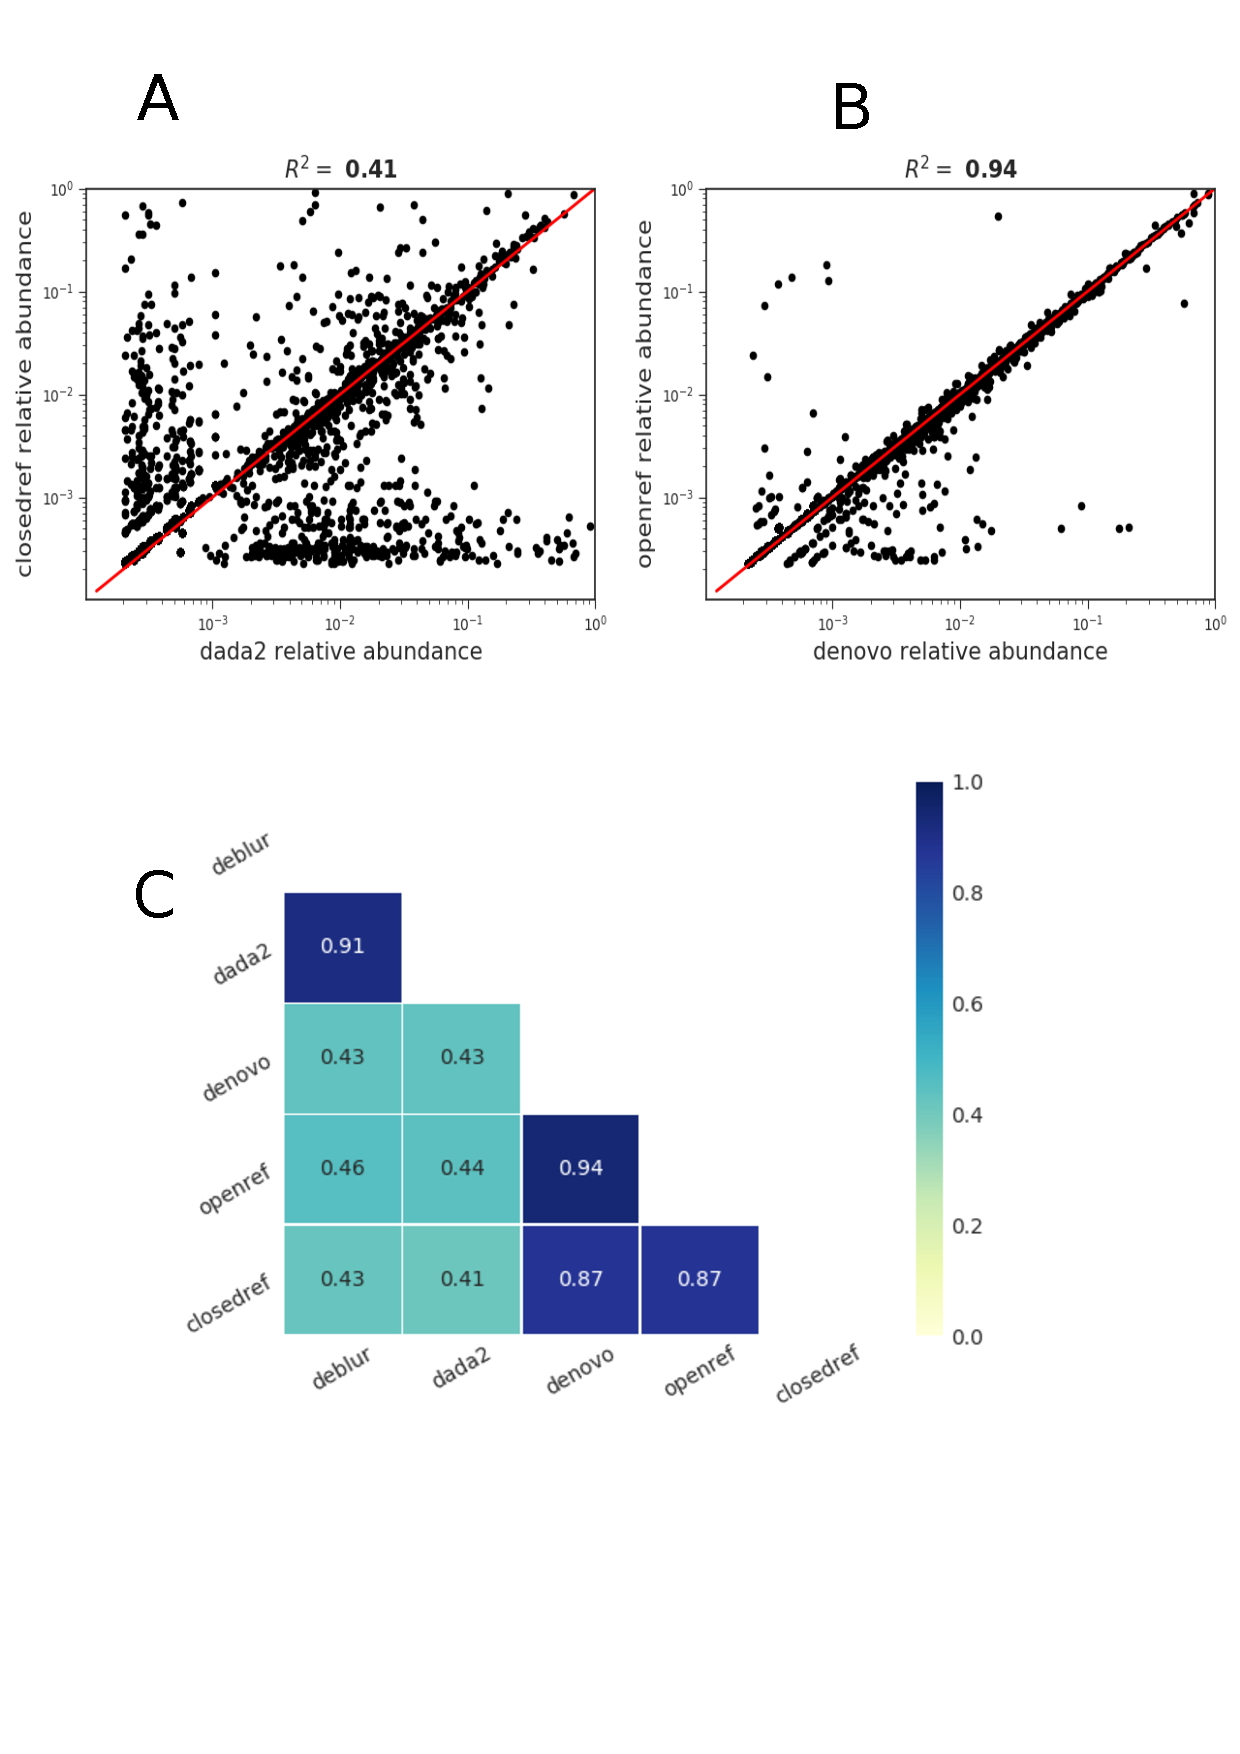
\includegraphics[width=15.8cm]{otu_corr_full.pdf}
      \caption{
        \textbf{Comparison of various denoising and clustering algorithms used in the pipeline}.
        (A, B) Correlation of the abundances of the taxa that are common between the count matrices created by two different methods.
        (A) The best correlation (most similar methods) is between open-reference and denovo.
        (B) The worst correlation (least similar methods) is between open-reference and dada2.
        (C) A heatmap showing the $\mathrm{R}^2$ of all pairwise comparisons of the methods.
      }
      \label{fig:otu_correlations}
    \end{center}
  \end{figure}

  \begin{figure}[h]
    \begin{center}
      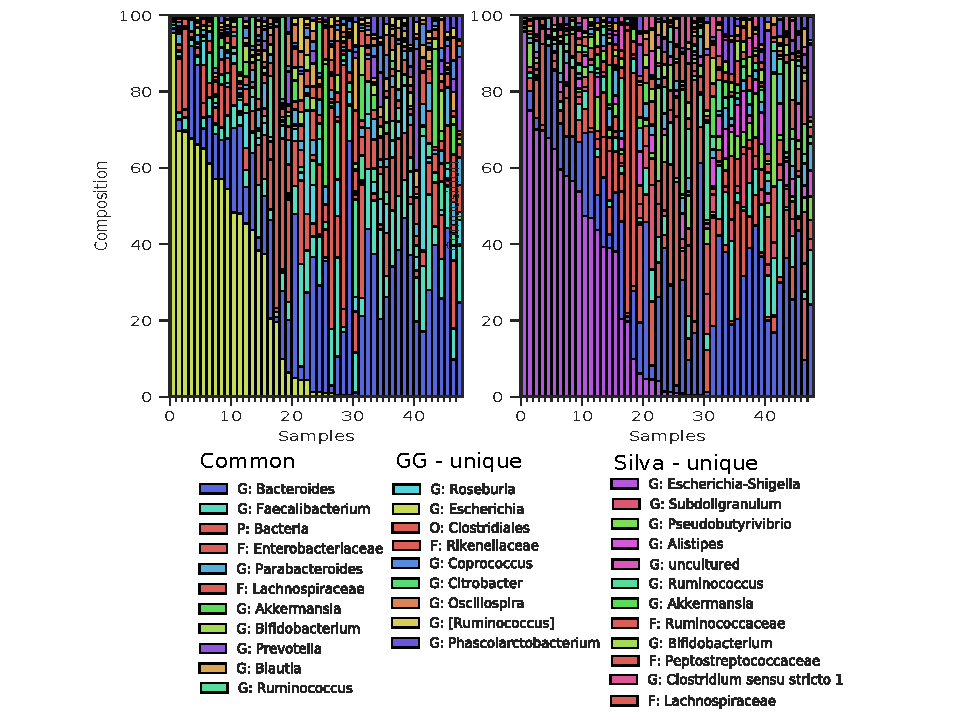
\includegraphics[width=17.8cm]{tax_comp_full.pdf}
      \caption{\textbf{Taxonomy composition of the 20 most abundant genera predicted using different taxonomy references databases}. NOTE: I will replace the legend with the taxonomy tree}
      \label{fig:tax_comp}
    \end{center}
  \end{figure}

  \begin{figure}[h]
    \begin{center}
      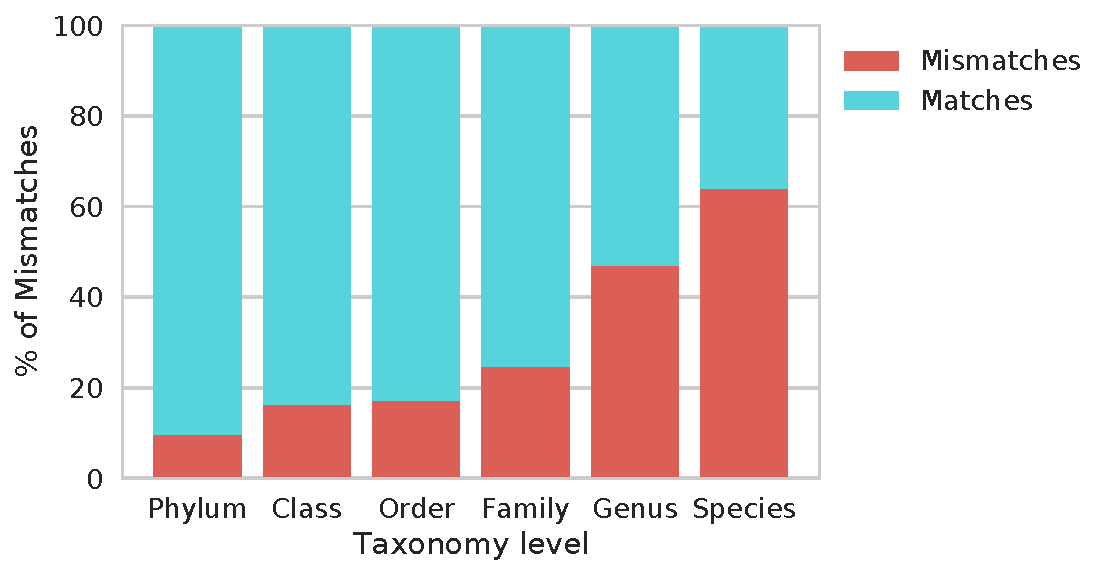
\includegraphics[width=15.8cm]{tax_distance_deblur.pdf}
      \caption{\textbf{Average percentage of mismatches in taxonomy assignment at various taxonomy levels}. NOTE: I will include a boxplot of the weighted distance in the taxonomy tree}
      \label{fig:otu_correlations}
    \end{center}
  \end{figure}

  \begin{figure}[h]
    \begin{center}
      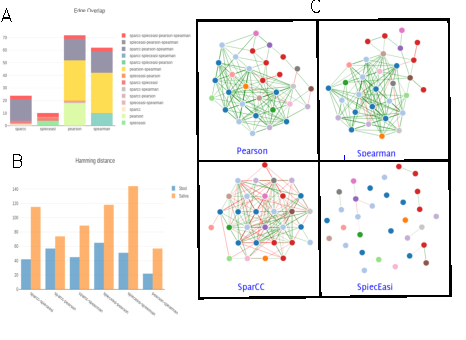
\includegraphics[width=17.8cm]{net_inference_comparison.pdf}
      \caption{
        \textbf{Networks generated using different network inference methods}.
        The four different networks generated by different network inference methods are very dissimilar (C).
        (A) The overlaps between the edges among the network5 generated is shown. The number of edges that are common to all networks are very low (5).
        (B) The hamming distance between the networks is shown. The similarity between various methods was found to vary with the data-source used.
      }
      \label{fig:network_comparison}
    \end{center}
  \end{figure}


  \begin{figure}[h]
    \begin{center}
      %\includegraphics[width=17.8cm]{../figures/network_comparison.pdf}
      \caption{\textbf{Core network captures known interactions in vaginal microbiota.} \textbf{a} Core network, obtained by taking the intersection between all the different pipelines. \textbf{b} Vaginal microbiota network as determined by XXX.}
      \label{fig:network_comparison}
    \end{center}
  \end{figure}
